%==============================================================================
%  Symposium poster  --  40 in (W) x 30 in (H)  landscape
%  Project: Constraining a Yukawa fifth force with Juno's orbit at Jupiter
%  Build:   pdflatex poster.tex   (run twice)
%
%  Board size 40" W x 30" H  ==  101.6 cm x 76.2 cm.
%  Uses beamerposter with size=custom so the geometry matches the board exactly.
%==============================================================================
\documentclass[final]{beamer}

% --- Poster geometry: 40in x 30in = 101.6cm x 76.2cm, landscape ----------------
\usepackage[orientation=landscape,size=custom,width=101.6,height=76.2,scale=1.35]{beamerposter}

\usepackage[utf8]{inputenc}
\usepackage[T1]{fontenc}
\usepackage{lmodern}
\usepackage{amsmath,amssymb}
\usepackage{graphicx}
\usepackage{booktabs}
\usepackage{ragged2e}
\graphicspath{{figures/}}

%==============================================================================
%  Colour + block theme  --  Brown University brand palette
%  (official Visual Identity: Red #ED1C24, Brown #4E3629, Gold #FFC72C)
%==============================================================================
\usepackage{tikz}
\definecolor{brownred}{HTML}{ED1C24}    % Brown University red (primary)
\definecolor{brownseal}{HTML}{4E3629}   % Brown University seal brown
\definecolor{browngold}{HTML}{FFC72C}   % Brown University gold (accent)
\definecolor{browngray}{HTML}{98A4AE}   % Brown University gray (accent)
\definecolor{lightgray}{RGB}{244,241,239}

\setbeamercolor{background canvas}{bg=white}
\setbeamercolor{block title}{fg=white,bg=brownred}
\setbeamercolor{block body}{fg=black,bg=lightgray}
\setbeamercolor{block alerted title}{fg=white,bg=brownseal}
\setbeamercolor{block alerted body}{fg=black,bg=lightgray}

%--- Official Brown Department of Physics logo (two-color stacked) --------------
% White-flattened version so the logo never renders on a black/transparent box.
\newcommand{\brownwordmark}{
\includegraphics[width=0.82\linewidth]{figures/brown_physics_logo_white.png}}

\setbeamerfont{block title}{size=\large,series=\bfseries}
\setbeamertemplate{caption}[numbered]
\setbeamertemplate{navigation symbols}{}

% Rounded blocks with a coloured title bar
\setbeamertemplate{block begin}{
  \begin{beamercolorbox}[colsep*=0ex,dp=0.6ex,center]{block title}
    \vskip0.4ex\usebeamerfont{block title}\insertblocktitle\vskip0.4ex
  \end{beamercolorbox}
  \nointerlineskip
  \usebeamerfont{block body}
  \begin{beamercolorbox}[colsep*=0ex,vmode]{block body}
    \vskip0.6ex\begin{minipage}{0.96\textwidth}\justifying
}
\setbeamertemplate{block end}{
    \end{minipage}\vskip0.6ex
  \end{beamercolorbox}\vskip1.6ex
}
\setbeamertemplate{block alerted begin}{
  \begin{beamercolorbox}[colsep*=0ex,dp=0.6ex,center]{block alerted title}
    \vskip0.4ex\usebeamerfont{block title}\insertblocktitle\vskip0.4ex
  \end{beamercolorbox}
  \nointerlineskip
  \usebeamerfont{block body}
  \begin{beamercolorbox}[colsep*=0ex,vmode]{block alerted body}
    \vskip0.6ex\begin{minipage}{0.96\textwidth}\justifying
}
\setbeamertemplate{block alerted end}{
    \end{minipage}\vskip0.6ex
  \end{beamercolorbox}\vskip1.6ex
}

\newlength{\colw}
\setlength{\colw}{0.3\paperwidth}
\newcommand{\sepwidth}{0.02\paperwidth}

%==============================================================================
%  Title block content
%==============================================================================
\title{Updating Constraints on Beyond-the-Standard-Model Gravity using NASA's Juno Mission Data}
\author{Eashan Iyer, Ash Lassonde, Praniti Singh, JiJi Fan}
\institute{Department of Physics, Brown University}

\begin{document}
\begin{frame}[t]

%------------------------------------------------------------------ Header ------
% White header so the official two-color Brown logo reads cleanly; the red
% scheme is carried by the title text, the accent rule, and all block titles.
\begin{beamercolorbox}[wd=\paperwidth,sep=1.2ex]{background canvas}
  \vskip0.4ex
  \begin{columns}[c]
    \begin{column}{0.20\paperwidth}\centering
      \brownwordmark
    \end{column}
    \begin{column}{0.78\paperwidth}\centering
      {\veryHuge\bfseries\color{brownred}Updating Constraints on Beyond-the-Standard-Model Gravity using NASA's Juno Mission Data\par}
      \vskip1.2ex
      {\Large\bfseries\color{brownseal}%
        Eashan Iyer\textsuperscript{1},\;
        Ash Lassonde\textsuperscript{1},\;
        Praniti Singh\textsuperscript{1},\;
        JiJi Fan\textsuperscript{1}\par}
      \vskip0.5ex
      {\large\color{brownseal}\textsuperscript{1}Department of Physics, Brown University
        \quad\textbullet\quad Symposium 2026\par}
    \end{column}
  \end{columns}
  \vskip0.4ex
\end{beamercolorbox}
% thick red accent rule under the header
\vskip0.4ex
\begin{beamercolorbox}[wd=\paperwidth,ht=1.1ex,dp=0ex]{block title}\end{beamercolorbox}
\vskip2ex

%------------------------------------------------------------ Three columns -----
\begin{columns}[t]

%======================= LEFT COLUMN ==========================================
\begin{column}{\colw}

  \begin{block}{Motivation: gravity as a probe of new physics}
    Many extensions of the Standard Model predict a \textbf{Yukawa-type ``fifth
    force''} between masses, adding to Newtonian gravity a potential
    \[
      V(r)\;\propto\;\alpha\,\frac{e^{-r/\lambda}}{r},
    \]
    with \textbf{coupling strength} $\alpha$ and \textbf{range}
    $\lambda=\hbar c/m_\ast$ set by a hypothetical mediator of mass $m_\ast$.
    Such a force would slowly rotate a planet's orbit
    (\textbf{apsidal precession}). \\[0.5ex]
    NASA's \textbf{Juno} spacecraft has measured Jupiter's gravity field to
    exquisite precision over dozens of close ``perijove'' passes. We ask:
    \emph{how large a fifth force is still allowed by what Juno sees?}
  \end{block}

  \begin{block}{Method: from a covariance matrix to a bound}
    A fifth force and Jupiter's own gravity harmonics $J_n$ both drive the drift
    $\Delta\omega$ of the orbit's argument of perijove. The
    gravity-field uncertainty therefore sets how large a fifth-force signal could
    hide in the data. We propagate the measured gravity covariance $C$ into the
    precession uncertainty (Singh et al.\ 2025, eq.~3.5):
    \[
      \sigma_\omega=\sqrt{\mathbf{g}^{\mathsf T}\,C\,\mathbf{g}},
      \qquad
      \mathbf{g}=\frac{\partial\langle\Delta\omega\rangle}{\partial(GM,\,J_2\ldots J_N)}.
    \]
    Requiring the fifth-force drift not to exceed $2\sigma_\omega$ gives a
    \textbf{95\% C.L.\ bound}
    \[
      \boxed{\;\alpha_{\rm limit}(\lambda)=\dfrac{2\,\sigma_\omega}{|g(\lambda)|}\;},
      \qquad g(\lambda)=\frac{\langle\Delta\omega\rangle}{\alpha},
    \]
    where $g(\lambda)$ uses a \textbf{finite-size} Jupiter (radial density
    integral). The region \emph{above} $\alpha_{\rm limit}(\lambda)$ is excluded.
  \end{block}

  \begin{block}{Pipeline}
    \centering
    \footnotesize
    \begin{minipage}{0.95\textwidth}\ttfamily\raggedright
    gravity covariance $C$ [GM,\,J2..JN]\\
    \quad$+$ Appendix-B derivatives $\partial\langle\Delta\omega\rangle/\partial J_l$\\
    \quad$+$ GR term $6\pi\mu/[a(1-e^2)c^2]$\\
    $\Rightarrow\ \sigma_\omega=\sqrt{\mathbf{g}^{\mathsf T}C\,\mathbf{g}}$\\[0.5ex]
    Jupiter $\rho(r)\ \Rightarrow\ g(\lambda)$ (Yukawa, finite size)\\[0.5ex]
    $\Rightarrow\ \alpha_{\rm limit}=2\sigma_\omega/|g(\lambda)|\ \Rightarrow$ exclusion curve
    \end{minipage}
    \vskip1ex
    \raggedright\normalsize
    Implemented in Python (NumPy/Matplotlib); validated against the published
    Juno curve of Singh et al., \emph{JHEP} 01 (2025) 098.
  \end{block}

\end{column}

%======================= MIDDLE COLUMN ========================================
\begin{column}{\colw}

  \begin{block}{The excluded region (reproduction of Singh et al.\ 2025)}
    \centering
    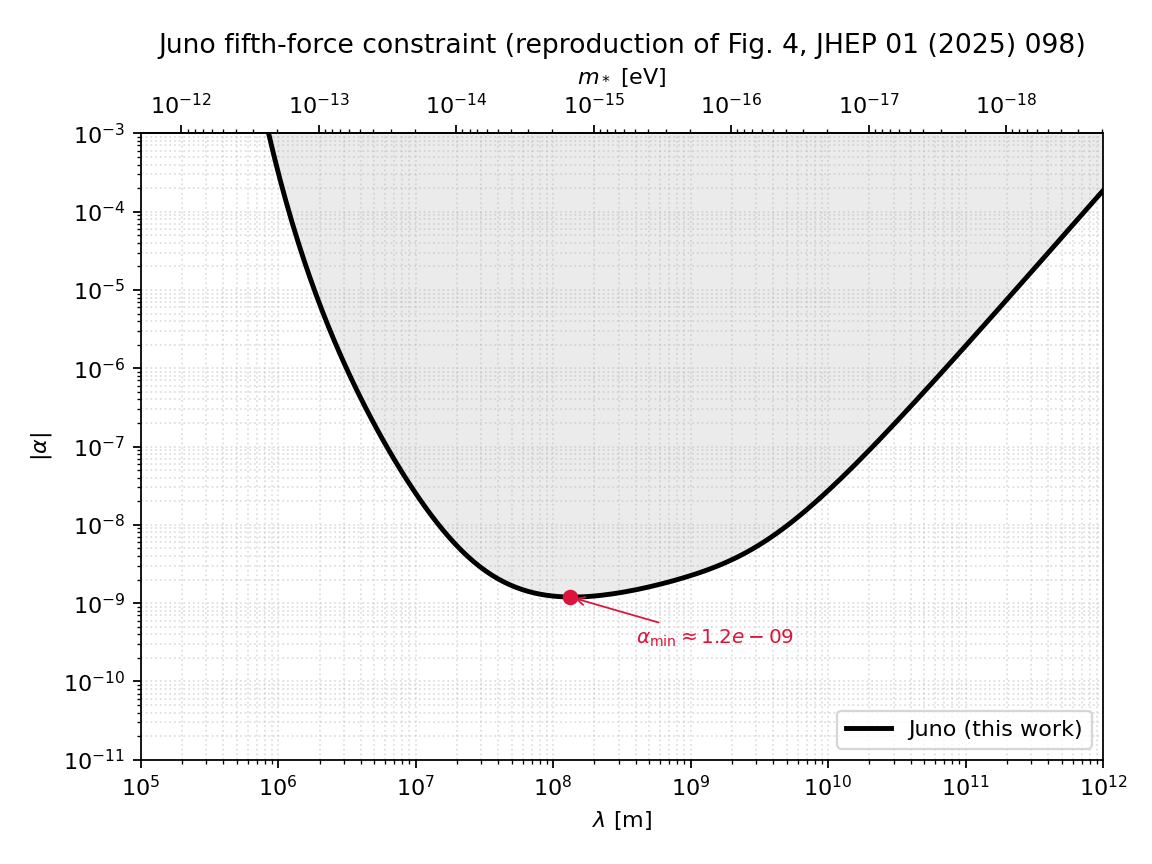
\includegraphics[width=0.98\textwidth]{figure4_juno.png}
    \vskip0.5ex
    \raggedright\small
    \textbf{Fig.~1.} Juno 95\% C.L.\ bound on a fifth force. The strongest limit,
    $\alpha_{\min}\approx1.2\times10^{-9}$, sits at
    $\lambda\sim1.3\times10^{8}\,$m ($\sim$1--2 Jupiter radii). Everything above
    the curve is excluded. This reproduces the black Juno curve of the reference
    paper ($\sigma_\omega\approx9.3\times10^{-10}$ vs.\ $\approx9\times10^{-10}$).
  \end{block}

  \begin{block}{Which harmonics matter?}
    \centering
    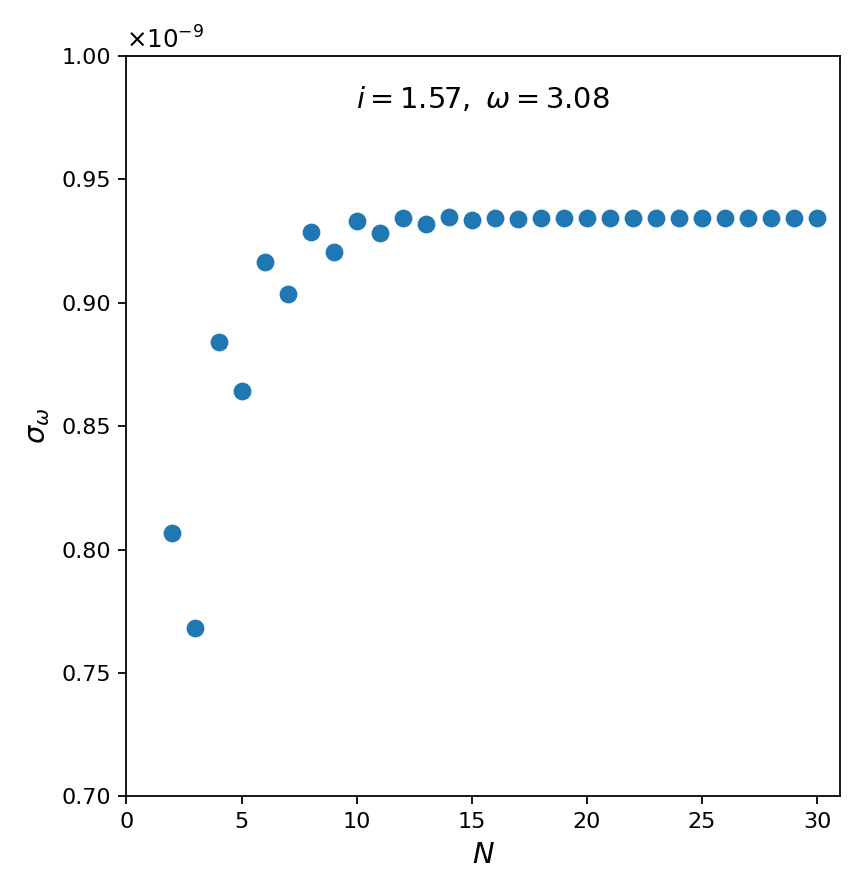
\includegraphics[width=0.80\textwidth]{figure3_right.png}
    \vskip0.5ex
    \raggedright\small
    \textbf{Fig.~2.} $\sigma_\omega$ vs.\ harmonic truncation $N$ (keep
    $J_2\ldots J_N$). The bound is set by \textbf{low-degree} gravity: because
    $|\partial\Delta\omega/\partial J_l|\propto(R_J/a)^l$, sensitivity is
    dominated by $J_2$ and $\sigma_\omega$ plateaus once $N\gtrsim12$. The
    gravitational parameter $GM$ contributes $<0.1\%$.
  \end{block}

\end{column}

%======================= RIGHT COLUMN =========================================
\begin{column}{\colw}

  \begin{alertblock}{Result: newer Juno data tighten the bound}
    \centering
    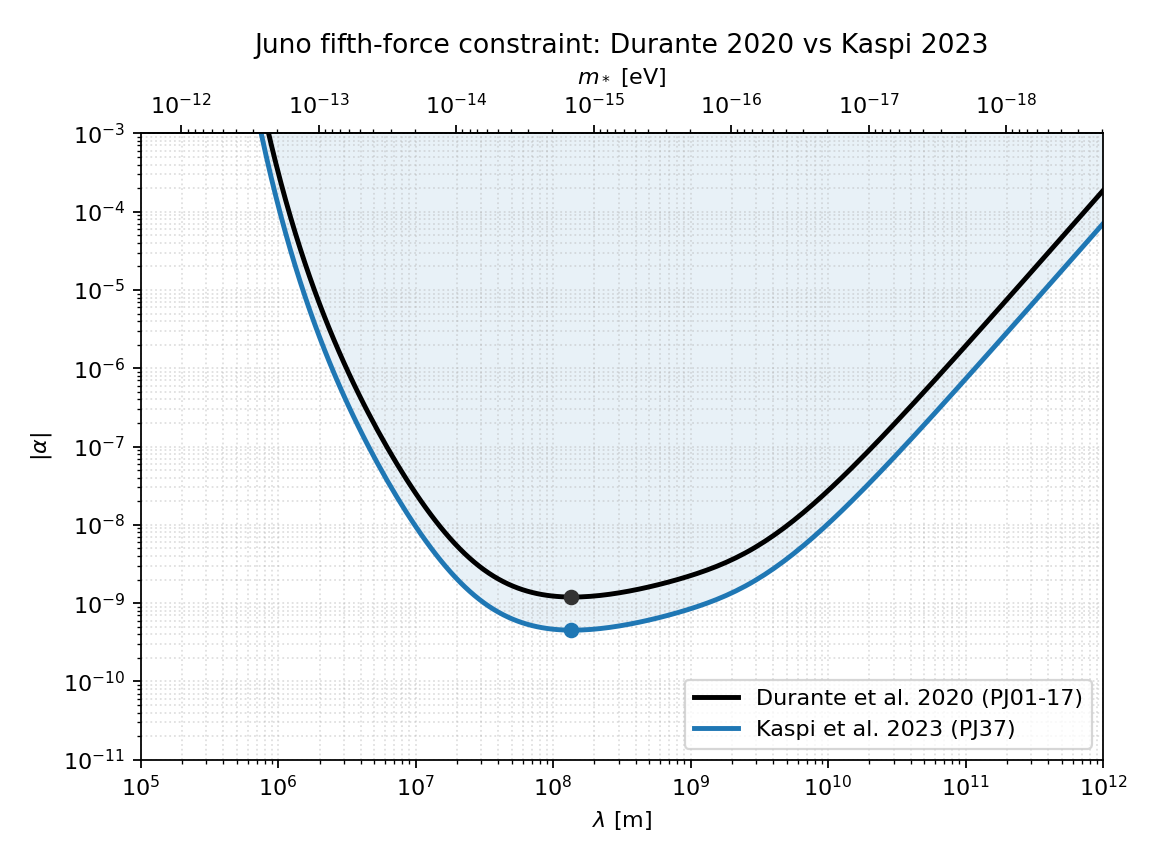
\includegraphics[width=0.98\textwidth]{figure4_comparison.png}
    \vskip0.5ex
    \raggedright\small
    \textbf{Fig.~3.} Updating the gravity solution from \textbf{Durante et al.\
    2020} (PJ01--17) to \textbf{Kaspi et al.\ 2023} (PJ37) lowers $\sigma_\omega$
    and pushes the exclusion curve down --- a \textbf{2.65$\times$} tightening in
    a same-basis comparison.
  \end{alertblock}

  \begin{block}{A methodological caveat: normalization basis}
    \centering
    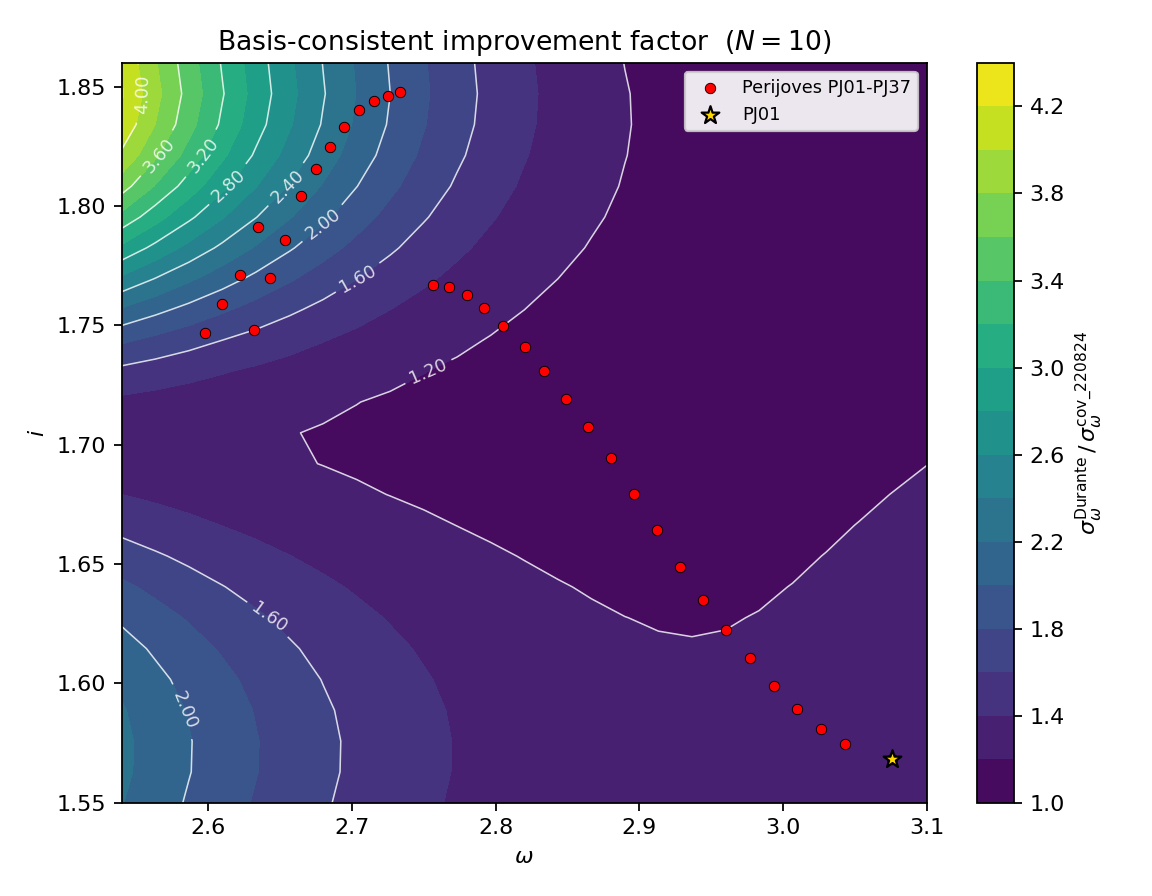
\includegraphics[width=0.86\textwidth]{sigma_omega_iw_ratio.png}
    \vskip0.5ex
    \raggedright\small
    \textbf{Fig.~4.} Improvement factor
    $\sigma_\omega^{\rm Durante}/\sigma_\omega^{\rm cov\_220824}$ across the
    $(\omega,i)$ orbit plane. When each covariance is used in its \emph{verified}
    normalization basis, the gain at Juno's geometry (PJ01, star) is a more modest
    \textbf{$\sim$1.3$\times$}, not 2.65$\times$. Comparing covariance matrices
    requires matching the harmonic normalization convention --- a subtle but
    decisive point.
  \end{block}

  \begin{block}{Conclusions}
    \begin{itemize}
      \item Juno's orbital precession excludes fifth forces with
            $\alpha\gtrsim10^{-9}$ near $\lambda\sim10^{8}\,$m.
      \item The bound is driven by \textbf{low-degree gravity harmonics},
            especially $J_2$; $\sigma_\omega$ saturates by $N\sim4$--$12$.
      \item Modern Juno solutions (37 perijoves) strengthen the limit by
            \textbf{$\sim$1.3--2.7$\times$}, depending on how covariances are compared.
      \item Careful \textbf{normalization bookkeeping} is essential when reusing
            published gravity covariances for particle-physics limits.
    \end{itemize}
    \vskip0.5ex
    {\footnotesize\textbf{References:} Singh et al., \emph{JHEP} 01 (2025) 098
    [arXiv:2409.10616]; Durante et al., \emph{GRL} 47 (2020); Kaspi et al.,
    \emph{Nat.\ Astron.} 7, 1463 (2023).}
  \end{block}

\end{column}

\end{columns}

%------------------------------------------------------------------ Footer ------
\vfill
\begin{beamercolorbox}[wd=\paperwidth,sep=0.6ex]{block title}
  \centering\small
  Reproduction and extension of Singh et al.\ (2025) \textbullet\ Data: Durante (2020) \& Kaspi (2023) Juno gravity covariances \textbullet\ Code in Python (NumPy/Matplotlib)
\end{beamercolorbox}

\end{frame}
\end{document}
